% =====================================================================
% TA-IND-01 — Informe Académico Individual (Aplicaciones Distribuidas)
% Análisis crítico de ClickHouse como sistema distribuido y su
% comparación con Elasticsearch
%
% Compilar desde la carpeta documento/, en este orden:
%   pdflatex TA-IND-01_Apunte_Washington.tex
%   biber TA-IND-01_Apunte_Washington
%   pdflatex TA-IND-01_Apunte_Washington.tex
%   pdflatex TA-IND-01_Apunte_Washington.tex
% =====================================================================
\documentclass[12pt,a4paper]{article}

\usepackage[T1]{fontenc}
\usepackage[utf8]{inputenc}
\usepackage[american,spanish,es-tabla,es-nodecimaldot,es-noquoting]{babel}
\usepackage{lmodern}
\usepackage[margin=2.5cm]{geometry}
\usepackage{graphicx}
\graphicspath{{figuras/}{../capturas/}{../anexos/}}
\usepackage{booktabs}
\usepackage{tabularx}
\usepackage{float}
\usepackage{caption}
\usepackage{xcolor}
\usepackage{listings}
\lstset{basicstyle=\ttfamily\small, breaklines=true, frame=single, columns=fullflexible}
\usepackage{csquotes}
% Estilo IEEE (biblatex-ieee v1.4g incluido en esta carpeta: ieee.bbx, ieee.cbx)
\usepackage[backend=biber,style=ieee,autolang=other,maxcitenames=6]{biblatex}
\addbibresource{referencias.bib}
\renewcommand*{\bibfont}{\small}
% Evita cortar un DOI justo después de un guion
\setcounter{biburlbigbreakpenalty}{10000}
\usepackage[titletoc,title]{appendix}
\addto\captionsspanish{%
  \renewcommand{\appendixname}{Anexo}%
  \renewcommand{\appendixtocname}{Anexos}%
  \renewcommand{\appendixpagename}{Anexos}%
}
\usepackage[hidelinks]{hyperref}
\usepackage{xurl}

\begin{document}

% ---------------------------------------------------------------------
% CARÁTULA
% ---------------------------------------------------------------------
\begin{titlepage}
  \centering
  {\large\bfseries UNIVERSIDAD TÉCNICA ESTATAL DE QUEVEDO\par}
  \vspace{0.3cm}
  {\large Facultad de Ciencias de la Computación y Diseño Digital\par}
  \vspace{0.2cm}
  {\large Carrera de Software\par}
  \vspace{1.5cm}
  {\Large\bfseries Aplicaciones Distribuidas\par}
  \vspace{0.4cm}
  {\large TA-IND-01 — Informe Académico Individual\par}
  \vspace{1.5cm}
  {\LARGE\bfseries Análisis crítico de ClickHouse como sistema distribuido y su comparación con Elasticsearch\par}
  \vfill
  \begin{tabular}{rl}
    \textbf{Estudiante:} & Washington German Apunte Pazmiño \\
    \textbf{Nivel y paralelo:} & Séptimo nivel, paralelo B \\
    \textbf{Docente:} & Gleiston Guerrero Ulloa, PhD \\
    \textbf{Fecha:} & 14 de noviembre de 2026 \\
  \end{tabular}
  \par\vspace{1cm}
  \textbf{Repositorio:}\par
  \url{https://github.com/Washinton-Apunte/TA-IND-01-ClickHouse}
\end{titlepage}

% ---------------------------------------------------------------------
% RESUMEN
% ---------------------------------------------------------------------
\pagenumbering{roman}
\begin{abstract}
Este informe analiza ClickHouse, una base de datos analítica de código
abierto, como sistema distribuido, y lo compara con Elasticsearch.
Apliqué los conceptos de la Unidad~1 (transparencias de distribución,
teorema CAP y su extensión PACELC, modelos de comunicación y tolerancia
a fallos) a partir de artículos científicos y de un experimento propio:
un clúster con dos réplicas y tres nodos de ClickHouse Keeper, montado
con Docker en mi computadora. En cuatro pruebas detuve la copia entre
réplicas, apagué una réplica, dejé a Keeper sin mayoría y medí la
latencia de escritura con y sin quórum. Los resultados muestran que, por
defecto, ClickHouse prioriza la disponibilidad y la latencia: aceptó
escrituras con una réplica caída, y una réplica llegó a responder con
46~segundos de atraso. Exigir el quórum de dos réplicas garantizó la
consistencia, pero multiplicó por 4,1 el tiempo promedio de escritura.
Sin mayoría en Keeper, las tablas quedaron en solo lectura. Concluyo que
ClickHouse oculta dónde están los datos, pero no cuándo se actualizan, y
que es adecuado para analizar grandes volúmenes de datos, pero no para
sistemas transaccionales.
\end{abstract}

\tableofcontents
\newpage
\pagenumbering{arabic}


\section{Introducción}
Las empresas guardan y analizan cada vez más datos: registros de
servidores, métricas, eventos de usuarios. Necesitan consultarlos en
tiempo casi real, con muchas consultas al mismo tiempo y sin que el costo
se dispare. ClickHouse es una base de datos analítica (OLAP) de código
abierto diseñada para hacer análisis de alto rendimiento sobre conjuntos
de datos de escala de petabytes y con altas tasas de ingesta, y busca
responder en menos de un segundo~\cite{schulze2024}. Guarda los datos
por columnas, reparte las tablas en fragmentos (\emph{shards}) y las
replica en varios nodos, por lo que es un sistema distribuido.

ClickHouse se usa en producción en empresas de infraestructura de
Internet. Un ejemplo es Cloudflare, que lo usa en los sistemas que
generan la configuración de su servicio de gestión de bots. El 18 de
noviembre de 2025, un cambio de permisos en su clúster de ClickHouse
terminó provocando la peor caída de su red desde 2019, durante la cual
no pudo entregar buena parte del tráfico de sus clientes~\cite{cloudflare2025}.
Este incidente se analiza en la sección de tolerancia a fallos.

Elegí ClickHouse porque ya lo usé en un proyecto de la asignatura de
Construcción de Software, en el que trabajé con una tabla de más de
3~millones de registros y las consultas respondieron rápido. Además, es
libre y gratuito, no necesita licencia y puedo integrarlo con los
sistemas que he desarrollado. Eso también me permitió levantar un
clúster real en mi computadora y hacer mis propias pruebas.

Lo comparo con Elasticsearch, un motor de búsqueda y análisis
distribuido que también se usa para guardar y consultar grandes
volúmenes de registros~\cite{calderon2024}. Los dos sistemas comparten
casos de uso, pero resuelven la distribución de forma distinta, y quiero
ver en qué se diferencian en su funcionamiento y qué compromisos hace
cada uno.

\section{Arquitectura del sistema}
Un clúster de ClickHouse se organiza en fragmentos (\emph{shards}) y
réplicas. El fragmentado reparte una tabla en partes independientes
según una expresión, y la replicación mantiene varias copias de cada
fragmento para tener escalabilidad y disponibilidad~\cite{schulze2024}.
Para el experimento armé en mi computadora, con Docker Compose, el
clúster más pequeño que permite observar la replicación: un fragmento,
dos réplicas y tres nodos de coordinación. La Figura~\ref{fig:arquitectura}
muestra sus componentes.

\begin{figure}[htbp]
  \centering
  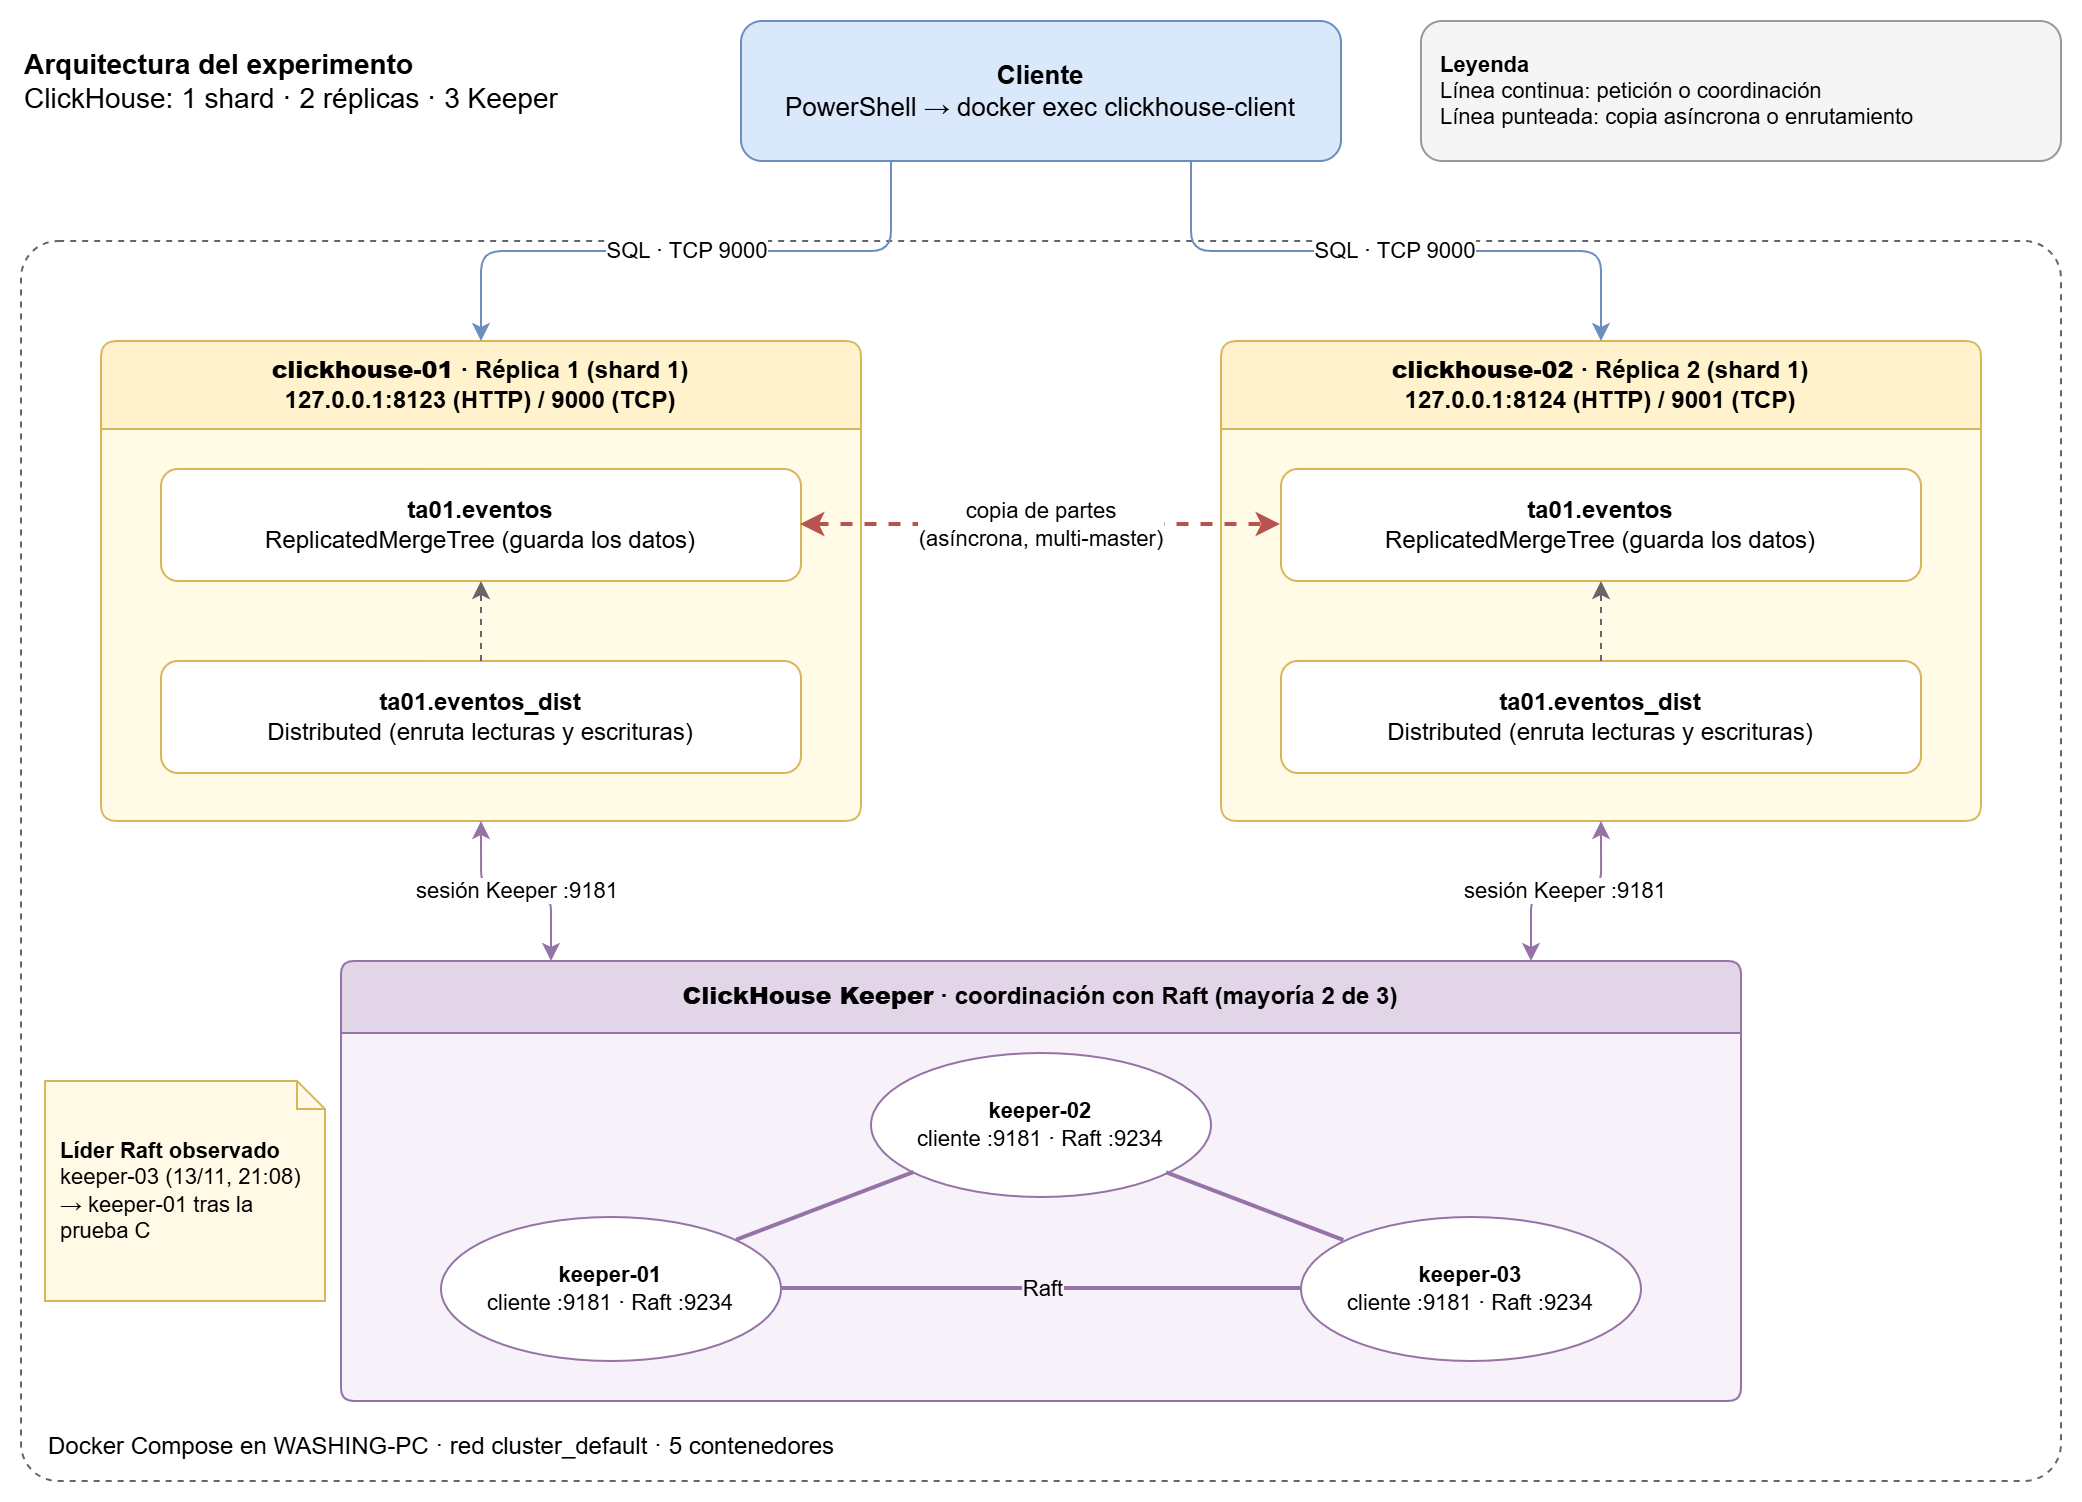
\includegraphics[width=\linewidth]{arquitectura.png}
  \caption{Arquitectura del clúster de ClickHouse usado en el experimento
  (diagrama propio elaborado en draw.io).}
  \label{fig:arquitectura}
\end{figure}

\paragraph{Réplicas.} Los servidores \texttt{clickhouse-01} y
\texttt{clickhouse-02} guardan copias idénticas de los datos para evitar
pérdidas si uno falla. La tabla \texttt{ta01.eventos} usa el motor
\texttt{ReplicatedMergeTree}, que coordina las réplicas con un esquema
\emph{multi-master}: cualquiera de las dos puede recibir escrituras y la
otra copia los cambios~\cite[p.~3732]{schulze2024}.

\paragraph{ClickHouse Keeper.} Tres nodos de Keeper coordinan la
sincronización entre las réplicas. Guardan el registro de replicación,
es decir, la lista ordenada de operaciones que cada réplica debe
aplicar, y usan el algoritmo de consenso Raft para ponerse de acuerdo
aunque falle uno de ellos~\cite[p.~3736]{schulze2024}. Por eso son tres: Raft
necesita una mayoría, y con tres nodos se puede perder uno sin dejar de
funcionar. En mi clúster, el líder de Raft fue al inicio
\texttt{clickhouse-keeper-03}.

\paragraph{Tabla Distributed.} La tabla \texttt{ta01.eventos\_dist} no
guarda datos: actúa como un enrutador que lee y escribe en todos los
servidores del clúster. Es el motor que ClickHouse usa para el
fragmentado transparente de los datos~\cite[p.~3732]{schulze2024}.

\paragraph{Comunicación entre componentes.} El cliente envía consultas
SQL a cada servidor por el protocolo nativo TCP (puerto 9000 dentro del
contenedor). Los servidores mantienen una sesión con Keeper (puerto
9181), y los nodos de Keeper se comunican entre sí con Raft (puerto
9234). Cuando una réplica recibe una inserción, la anota en el registro
de Keeper, y la otra réplica la descarga después de forma asíncrona.

\paragraph{Evolución del diseño.} El primer bosquejo, dibujado a mano
(Anexo~\ref{anexo:a}), era más simple y menos detallado: solo mostraba
el cliente, las dos réplicas y los tres nodos de Keeper. El diagrama
final integra los elementos que entendí al montar el clúster y hacer las
pruebas: la tabla Distributed, los puertos de cada comunicación, el
carácter asíncrono de la copia entre réplicas y el contenedor de Docker
Compose que agrupa todo.

\section{Análisis con los conceptos de la Unidad 1}

En esta sección uso los conceptos de la unidad para explicar el
comportamiento de ClickHouse. Me apoyo en los artículos citados y en lo
que observé en mis cuatro pruebas, que se detallan en la
sección~\ref{sec:experimento}.

\subsection{Transparencias de distribución}

Una transparencia oculta al usuario algún aspecto de la distribución,
de modo que el sistema se vea como si estuviera en una sola máquina. La
Tabla~\ref{tab:transparencias} resume cuáles ofrece ClickHouse.

\begin{table}[htbp]
  \centering
  \caption{Transparencias de distribución en ClickHouse.}
  \label{tab:transparencias}
  \small
  \begin{tabularx}{\linewidth}{@{}l l X@{}}
    \toprule
    \textbf{Transparencia} & \textbf{¿La ofrece?} & \textbf{Evidencia} \\
    \midrule
    Acceso & Sí & Se usa el mismo SQL para consultar una tabla local o la
      tabla Distributed que abarca todo el clúster. \\
    Ubicación & Parcial & La tabla Distributed oculta en qué fragmento está
      cada fila~\cite[p.~3732]{schulze2024}, pero cada réplica tiene su
      propia dirección y en mis pruebas elegí a qué servidor conectarme. \\
    Migración & No & La topología se define a mano en la configuración del
      clúster, así que los datos no se mueven solos entre fragmentos.
      Elasticsearch, en cambio, migra sus fragmentos
      automáticamente~\cite[p.~2377]{calderon2024}. \\
    Reubicación & Parcial & Una réplica que vuelve o que se agrega se pone al
      día copiando el estado de otra réplica~\cite[p.~3736]{schulze2024},
      mientras las demás siguen atendiendo (prueba~B). Pero la lista de
      servidores está fija en la configuración: si un servidor cambia de
      dirección, ni el cliente ni la tabla Distributed lo detectan solos. \\
    Replicación & Parcial & El usuario no administra las copias, pero puede
      leer datos viejos: en la prueba~A una réplica tenía 6 filas y la otra
      solo 1. \\
    Concurrencia & Sí & Cada consulta trabaja sobre una instantánea de las
      partes de la tabla (aislamiento por instantáneas), por lo que las
      inserciones paralelas no la afectan~\cite[p.~3736]{schulze2024}. \\
    Fallos & Parcial & La caída de una réplica no se notó al leer
      (prueba~B), pero sin mayoría en Keeper las escrituras fallaron
      (prueba~C). \\
    \bottomrule
  \end{tabularx}
\end{table}

La transparencia que más se rompe es la de replicación. Mientras hacía
las pruebas lo noté al leer los resultados: cada réplica respondía con
un número de filas distinto. El propio artículo de ClickHouse lo
reconoce: el registro de replicación se reproduce de forma asíncrona en
los demás nodos, por lo que las tablas replicadas solo son
eventualmente consistentes y un nodo puede leer temporalmente un estado
antiguo de la tabla~\cite[p.~3736]{schulze2024}. Es decir, ClickHouse
oculta \emph{dónde} están las copias, pero no oculta \emph{cuándo} se
actualizan.

\subsection{CAP y PACELC}

El teorema CAP plantea que, ante una partición de la red, un sistema
distribuido tolerante a fallos debe elegir entre disponibilidad y
consistencia. Una base de datos que prioriza la disponibilidad actualiza
sus réplicas de forma asíncrona y acepta una consistencia eventual; una
que prioriza la consistencia confirma la operación solo cuando todas las
réplicas están actualizadas~\cite[p.~3]{ferreira2024}. PACELC agrega que,
aun sin partición, el sistema debe elegir entre latencia y consistencia.

\paragraph{Con partición (P: A o C).} Por defecto, ClickHouse prioriza la
disponibilidad. En la prueba~B, con la réplica~2 apagada, el clúster
siguió aceptando escrituras: la fila~7 se guardó en una sola réplica y
la otra la recibió al volver. Pero el sistema permite pedir consistencia
en cada operación: con \texttt{insert\_quorum = 2}, la escritura de la
fila~8 se rechazó con el error 285 (\texttt{TOO\_FEW\_LIVE\_REPLICAS}),
porque había una sola réplica viva y se pedía la confirmación de dos.
El artículo de ClickHouse describe esta misma opción: la mayoría de las
operaciones se pueden ejecutar de forma síncrona hasta que un quórum de
nodos adopte el nuevo estado~\cite[p.~3736]{schulze2024}.

La capa de coordinación, en cambio, siempre prioriza la consistencia.
Keeper usa Raft y necesita una mayoría para aceptar cambios. En la
prueba~C, al apagar dos de los tres nodos, ClickHouse no se arriesgó a
guardar datos mal: la tabla pasó a solo lectura y la escritura nunca se
completó, aunque las lecturas siguieron funcionando.

\paragraph{Sin partición (E: L o C).} En condiciones normales, ClickHouse
prioriza la latencia. En la prueba~D, una escritura sin quórum tardó en
promedio 18,83~ms, y una que esperaba la confirmación de las dos
réplicas tardó 77,23~ms, unas cuatro veces más. Las réplicas se toman su
tiempo para copiar los datos, y esperar esa copia es exactamente lo que
cuesta la consistencia.

En resumen, con su configuración por defecto la capa de datos de
ClickHouse se comporta como un sistema \textbf{PA/EL}: si una réplica se
cae o queda aislada, las demás siguen aceptando lecturas y escrituras
mientras mantengan contacto con la mayoría de Keeper, y sin partición
prefiere responder rápido. Cada escritura puede pedir quórum y pasar a un
comportamiento \textbf{PC/EC}, pagando el costo en latencia que medí. Su
capa de coordinación, basada en Raft, es siempre CP: el lado de una
partición que se queda sin mayoría deja de aceptar escrituras.

\subsection{Modelos de comunicación}

ClickHouse combina varios modelos de comunicación:

\begin{itemize}
  \item \textbf{Cliente y servidor.} Me comunicaba con cada servidor
    mediante una conexión al puerto que usaba: el protocolo nativo sobre
    TCP en el puerto 9000 (también acepta HTTP en el 8123). Es una
    comunicación síncrona de petición y respuesta: el cliente espera el
    resultado de la consulta.
  \item \textbf{Entre réplicas.} La copia de datos no fue al mismo tiempo,
    sino después, de forma asíncrona. Cuando una réplica recibe una
    inserción, la anota en el registro de Keeper, y las demás leen ese
    registro y descargan la parte nueva desde la réplica que la
    tiene~\cite[p.~3736]{schulze2024}. Es un intercambio entre pares
    (\emph{multi-master}) coordinado por un servicio central, es decir,
    un modelo híbrido.
  \item \textbf{Entre los nodos de Keeper.} Se comunican con mensajes del
    algoritmo de consenso Raft (puerto 9234 en mi clúster) para elegir un
    líder y replicar el registro.
  \item \textbf{Inserciones asíncronas.} ClickHouse puede acumular las
    filas de varias inserciones pequeñas en un búfer y crear la parte
    nueva cuando el búfer se llena o pasa un tiempo
    límite~\cite[p.~3733]{schulze2024}. En mi servidor (versión
    26.10.4.207) este modo estaba activado por defecto
    (\texttt{async\_insert = 1}), como muestra la prueba~D.
  \item \textbf{Sockets, RPC y mensajería.} Toda la comunicación de mi
    clúster usa sockets TCP: el protocolo nativo del cliente (puerto 9000),
    la sesión con Keeper (9181) y Raft entre los nodos de Keeper (9234).
    Cada componente usa su propio protocolo, sin un marco de RPC general.
    ClickHouse tampoco es un sistema de mensajería, pero tiene motores de
    tabla virtuales para intercambiar datos con sistemas de publicación y
    suscripción como Kafka o RabbitMQ~\cite[p.~3732]{schulze2024}.
\end{itemize}

\subsection{Tolerancia a fallos}

\paragraph{Caída de una réplica.} Es el fallo que ClickHouse mejor
soporta. ClickHouse detecta qué réplicas están vivas mediante su sesión
con Keeper: en la prueba~B, \texttt{active\_replicas} bajó de 2 a 1 en
cuanto apagué la réplica. Al volver a encenderla, la réplica leyó el
registro de replicación, descargó la fila que le faltaba y quedó igual a
la otra sin que yo interviniera.

\paragraph{Pérdida de la mayoría en Keeper.} Tres nodos de Keeper
toleran la caída de uno. Con dos caídos, ClickHouse detectó que su
sesión había expirado (\texttt{is\_session\_expired = 1}) y puso la tabla
en solo lectura. La escritura no encontró a Keeper para registrarse:
tardó en cargar, quedó esperando 120~segundos y terminó con el
error 159 (\texttt{TIMEOUT\_EXCEEDED}). Al encender de nuevo los nodos,
Raft eligió un líder nuevo (\texttt{keeper-01}, cuando antes era
\texttt{keeper-03}) y la tabla volvió a aceptar escrituras sola.

\paragraph{Reintentos sin duplicados.} Cuando una escritura termina por
tiempo de espera, el cliente no sabe si se guardó o no. ClickHouse
resuelve este problema guardando en Keeper un resumen (\emph{hash}) de
las últimas partes insertadas e ignorando las que llegan repetidas, de
modo que el cliente puede reenviar el mismo lote sin
duplicarlo~\cite[p.~3736]{schulze2024}. En mi caso comprobé que la
escritura que falló en la prueba~C no se guardó.

\paragraph{Incidente real: Cloudflare, 18 de noviembre de 2025.} Cloudflare
usa ClickHouse para generar un archivo de configuración de su servicio
de gestión de bots. Ese día se aplicó un cambio de permisos que hizo
que los usuarios también pudieran ver los metadatos de las tablas
internas de la base de datos \texttt{r0}. Una consulta que no filtraba por nombre de base de datos
empezó a devolver filas duplicadas, el archivo duplicó su tamaño y
superó el límite de 200 características que aceptaba el sistema de
bots, que falló y devolvió errores HTTP~5xx. Como el cambio se estaba
aplicando de a poco en el clúster, cada cinco minutos se generaba un
archivo bueno o uno malo según la parte del clúster que respondía la
consulta, hasta que todos los nodos generaron el archivo erróneo~\cite{cloudflare2025}.

La lección que saco es que un sistema distribuido, si se configura o se
usa de forma inadecuada, deja de dar el servicio para el que fue
diseñado. La replicación protege contra la caída de un servidor, pero no
contra un error lógico: al contrario, lo propaga a todos los nodos.
Además, el incidente fue una falla de transparencia: una consulta que
asumía ver una sola copia lógica de los datos terminó viendo también las
tablas internas de la distribución.

\section{Experimentación propia}\label{sec:experimento}

\subsection{Entorno y procedimiento}

Monté el clúster en mi computadora (\texttt{WASHING-PC}, Windows con
Docker Desktop) usando la receta oficial de ClickHouse para un fragmento
con dos réplicas y tres nodos de Keeper, con las imágenes
\texttt{clickhouse/clickhouse-server} (versión 26.10.4.207) y
\texttt{clickhouse/clickhouse-keeper}. Todos los comandos, el script de
la prueba de latencia y los resultados exportados de
\texttt{system.query\_log} están en la carpeta \texttt{experimento} del
repositorio. En cada captura se ven mi usuario, el nombre de mi equipo y
la fecha y hora. La Tabla~\ref{tab:pruebas} resume las cuatro pruebas.

\begin{table}[htbp]
  \centering
  \caption{Resumen de las pruebas realizadas el 13/11/2026.}
  \label{tab:pruebas}
  \small
  \begin{tabularx}{\linewidth}{@{}l X X l@{}}
    \toprule
    \textbf{Prueba} & \textbf{Qué hice} & \textbf{Qué observé} &
      \textbf{Concepto} \\
    \midrule
    A & Detuve la copia hacia la réplica~2 e inserté 5 filas en la
      réplica~1. & La réplica~1 tenía 6 filas y la réplica~2 solo 1, con
      46~s de retraso. Al reanudar la copia, las dos quedaron con 6. &
      Consistencia eventual \\
    B & Apagué la réplica~2 e inserté sin quórum y con quórum de 2. &
      Sin quórum se aceptó; con quórum se rechazó (error 285). Al volver,
      la réplica~2 recibió la fila que le faltaba. & CAP y tolerancia a
      fallos \\
    C & Apagué 2 de los 3 nodos de Keeper. & La tabla quedó en solo
      lectura; la lectura funcionó y la escritura falló a los 120~s
      (error 159). Al volver, Raft eligió un líder nuevo. & Consenso
      (CP) \\
    D & Ejecuté 30 inserciones sin quórum y 30 con quórum de 2. & Con
      quórum, la escritura tardó unas cuatro veces más
      (Tabla~\ref{tab:latencia}). & PACELC \\
    \bottomrule
  \end{tabularx}
\end{table}

\subsection{Clúster en funcionamiento}

La Figura~\ref{fig:contenedores} muestra los cinco contenedores en
ejecución y la Figura~\ref{fig:keeper} el estado de los nodos de Keeper:
uno actúa como líder y los otros dos como seguidores, lo que confirma
que Raft eligió un líder al arrancar.

\begin{figure}[htbp]
  \centering
  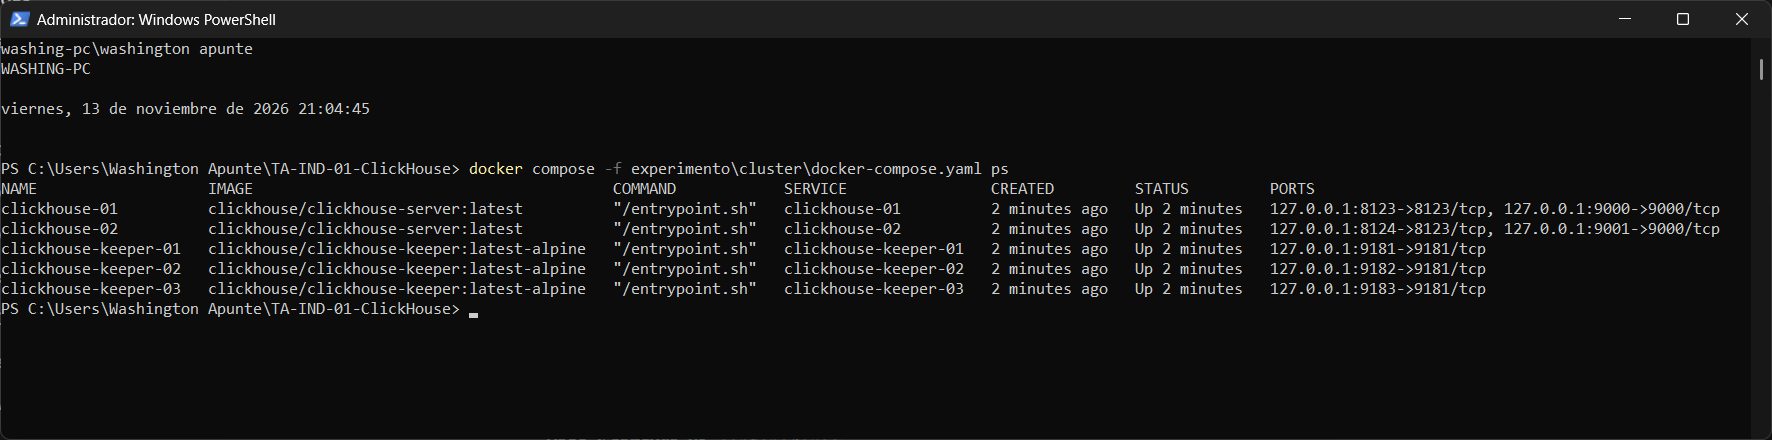
\includegraphics[width=0.9\linewidth]{01-contenedores.png}
  \caption{Los cinco contenedores del clúster en ejecución.}
  \label{fig:contenedores}
\end{figure}

\begin{figure}[htbp]
  \centering
  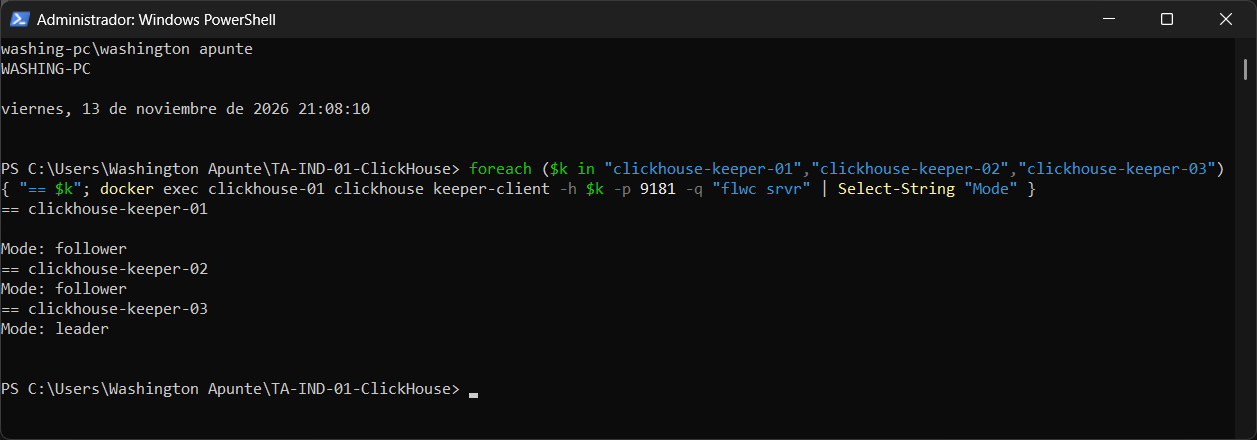
\includegraphics[width=0.9\linewidth]{03-keeper.png}
  \caption{Estado de los tres nodos de Keeper: un líder y dos seguidores.}
  \label{fig:keeper}
\end{figure}

\subsection{Prueba A: consistencia eventual}

Con \texttt{SYSTEM STOP FETCHES} impedí que la réplica~2 descargara datos
nuevos y luego inserté 5 filas en la réplica~1. Como muestra la
Figura~\ref{fig:pruebaA}, las dos réplicas respondieron con datos
distintos (6 y 1 filas), y la réplica~2 tenía una inserción pendiente
en su cola, con 46~segundos de retraso. Al reanudar la copia, la
réplica~2 se puso al día sola y las dos quedaron con 6 filas. Ambas
siguieron respondiendo todo el tiempo, aunque una con datos viejos: es
la consistencia eventual que describe el
artículo~\cite[p.~3736]{schulze2024}.

\begin{figure}[htbp]
  \centering
  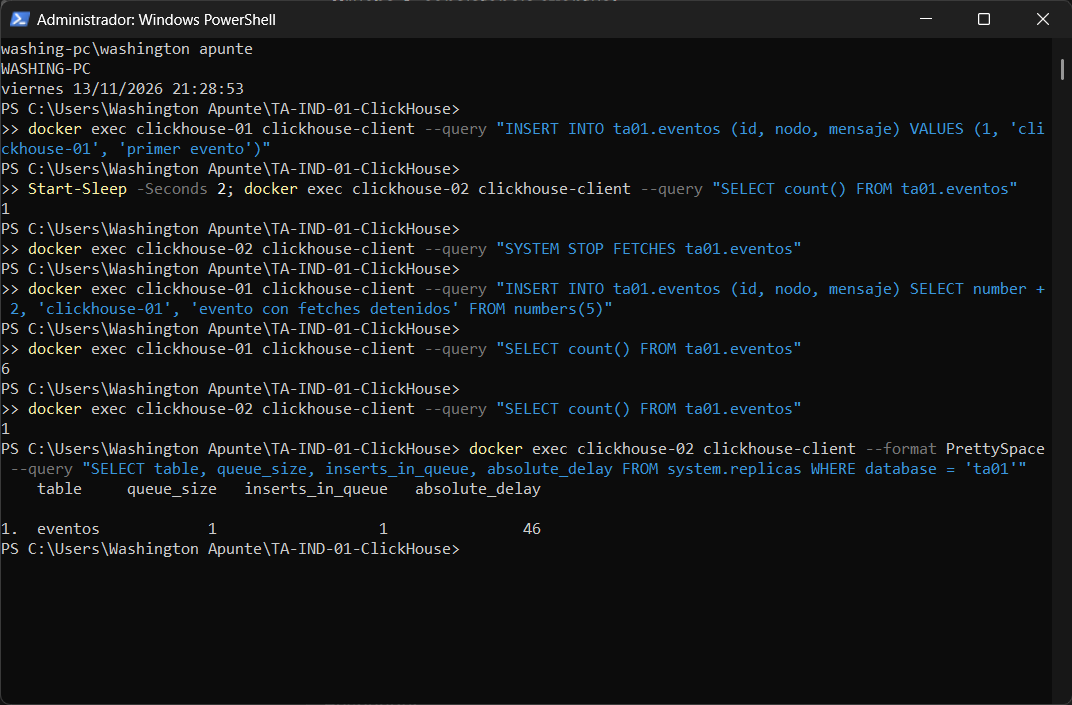
\includegraphics[width=0.9\linewidth]{05-prueba-a-retraso.png}
  \caption{Prueba A: con la copia detenida, la réplica 1 tiene 6 filas y
  la réplica 2 solo 1.}
  \label{fig:pruebaA}
\end{figure}

\subsection{Prueba B: caída de una réplica}

Apagué el contenedor \texttt{clickhouse-02}. La Figura~\ref{fig:pruebaB}
muestra que la escritura normal se aceptó, mientras que la que exigía
la confirmación de dos réplicas se rechazó con el error 285. Al encender
de nuevo la réplica, esta tenía las 7 filas: recibió la fila~7, escrita
mientras estaba apagada, y no la fila~8, que había sido rechazada. Esto
muestra los dos lados de CAP en una misma prueba: el mismo clúster puede
priorizar la disponibilidad o la consistencia según cómo se pida cada
escritura.

\begin{figure}[htbp]
  \centering
  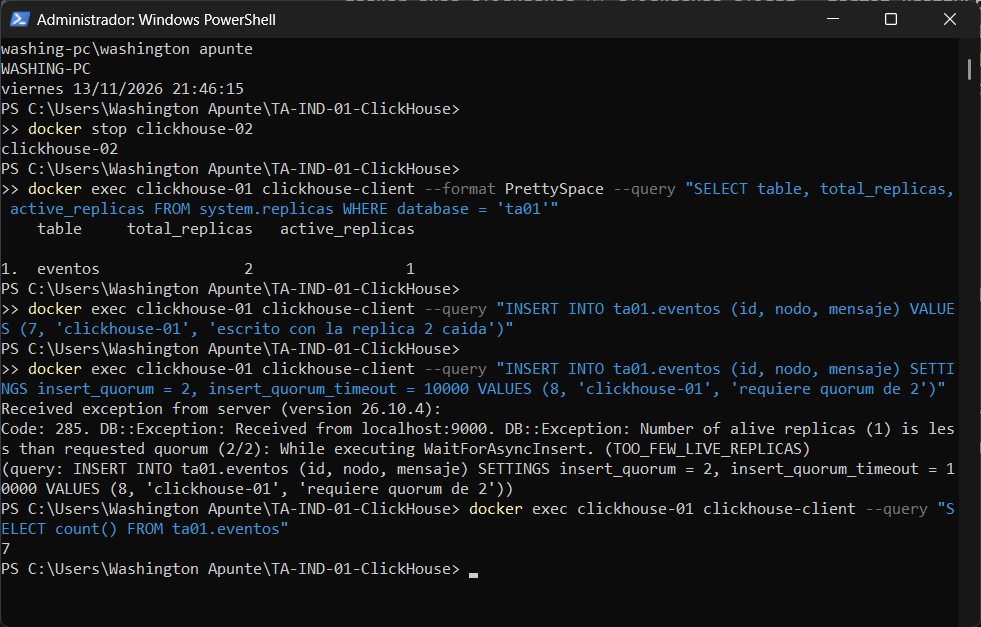
\includegraphics[width=0.9\linewidth]{07-prueba-b-replica-caida.png}
  \caption{Prueba B: con una réplica caída, la escritura con quórum de 2
  se rechaza (error 285).}
  \label{fig:pruebaB}
\end{figure}

\subsection{Prueba C: pérdida de la mayoría en Keeper}

Apagué \texttt{clickhouse-keeper-02} y \texttt{clickhouse-keeper-03}
(este último era el líder). Después de 40~segundos, la tabla estaba en
solo lectura y con la sesión expirada (Figura~\ref{fig:pruebaC}). La
lectura devolvió las 7 filas, pero la escritura quedó esperando y
terminó con el error 159 después de 120~segundos. Yo esperaba el error
\texttt{TABLE\_IS\_READ\_ONLY}, pero recibí un tiempo de espera agotado
porque mi versión de ClickHouse hace las inserciones de forma asíncrona
por defecto: la fila esperó en el búfer a que Keeper respondiera. Al
encender de nuevo los dos nodos, Raft eligió como líder a
\texttt{keeper-01} y la tabla volvió a aceptar escrituras. Comprobé que
la escritura fallida no se guardó.

\begin{figure}[htbp]
  \centering
  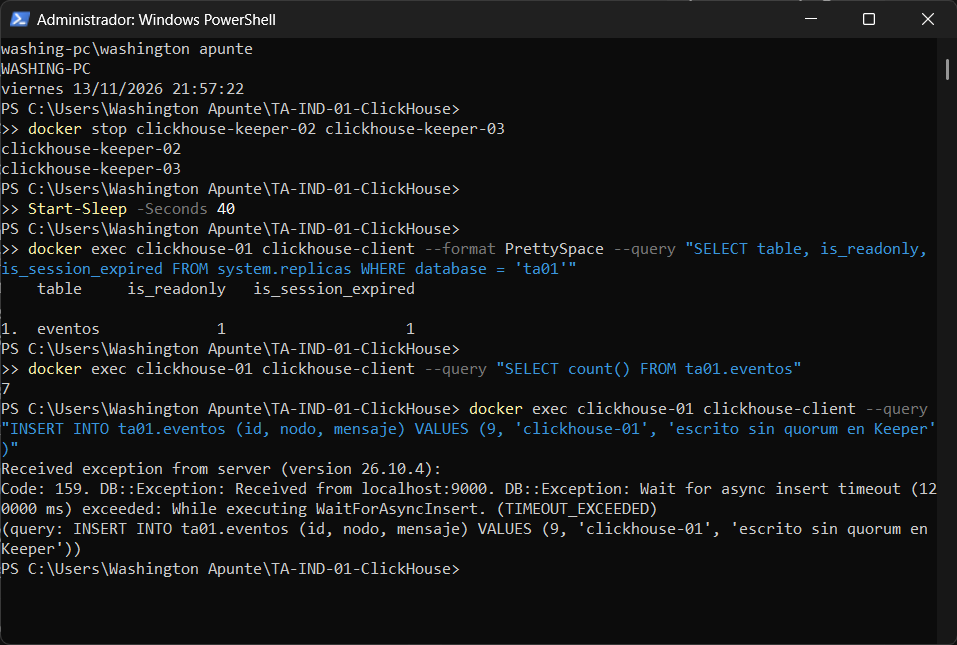
\includegraphics[width=0.9\linewidth]{09-prueba-c-sin-quorum.png}
  \caption{Prueba C: sin mayoría en Keeper, la tabla queda en solo
  lectura y la escritura no se completa.}
  \label{fig:pruebaC}
\end{figure}

\subsection{Prueba D: costo de la consistencia en latencia}

Ejecuté 30 inserciones sin quórum y 30 con \texttt{insert\_quorum = 2},
intercaladas, y medí su duración en \texttt{system.query\_log}. Desactivé
las inserciones asíncronas (\texttt{async\_insert = 0}) para que el
tiempo dependiera solo del quórum y no del búfer. La
Tabla~\ref{tab:latencia} y la Figura~\ref{fig:pruebaD} muestran el
resultado.

\begin{table}[htbp]
  \centering
  \caption{Duración de las inserciones (30 de cada tipo).}
  \label{tab:latencia}
  \begin{tabular}{@{}lrrrr@{}}
    \toprule
    \textbf{Modo} & \textbf{Promedio} & \textbf{Mediana} & \textbf{p95} &
      \textbf{Máximo} \\
    \midrule
    Sin quórum & 18,83~ms & 19~ms & 25~ms & 34~ms \\
    Quórum de 2 & 77,23~ms & 73~ms & 100~ms & 111~ms \\
    \bottomrule
  \end{tabular}
\end{table}

\begin{figure}[htbp]
  \centering
  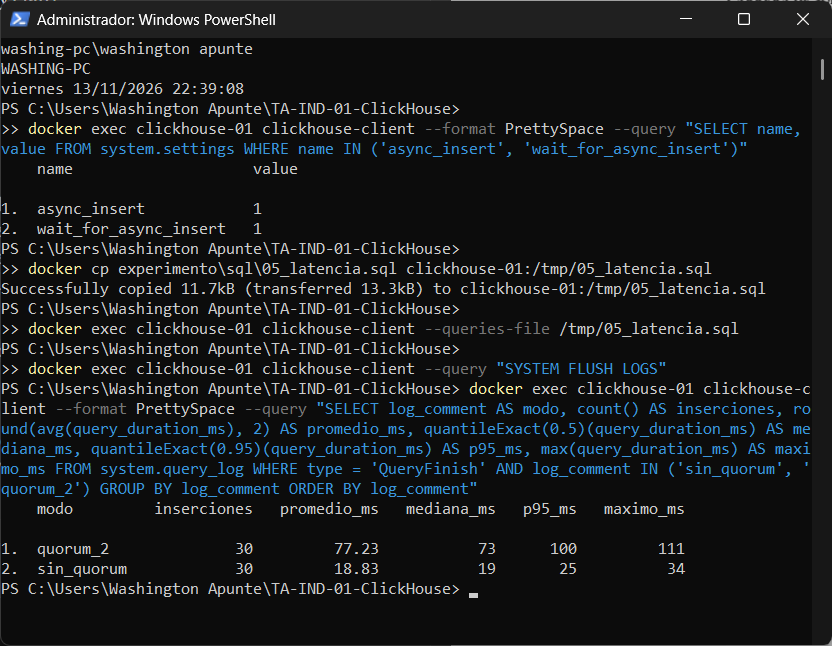
\includegraphics[width=0.9\linewidth]{11-prueba-d-latencia.png}
  \caption{Prueba D: configuración por defecto de las inserciones y
  latencia medida con y sin quórum.}
  \label{fig:pruebaD}
\end{figure}

Exigir la confirmación de las dos réplicas multiplicó el tiempo
promedio de escritura por 4,1. Este es el compromiso entre latencia y
consistencia que plantea PACELC, medido en mi propio equipo.

\subsection{Limitaciones}

Todos los contenedores corrían en la misma computadora, por lo que la
red entre réplicas era casi instantánea. En una red real, con servidores
en distintos lugares, el costo del quórum sería mayor. Además, la
muestra de la prueba~D es pequeña (30 inserciones por modo) y las
pruebas A, B y C se hicieron una sola vez, así que los tiempos son
ilustrativos y no un estudio de rendimiento.

\section{Ejemplos del entorno del estudiante}
Además del experimento, he observado como usuario el comportamiento de
varios sistemas distribuidos que uso a diario. Los relaciono con los
conceptos de la unidad.

\subsection{SGA de la UTEQ: disponibilidad bajo carga}
En una ocasión el SGA de la UTEQ no cargaba y no me permitía ingresar:
la página se quedaba cargando y no pasaba de ahí. Además, suele ponerse
lento en las matrículas, porque todos los estudiantes están obligados a
ingresar para matricularse, aunque se organicen por grupos de niveles en
diferentes horarios. Lo que más me ha pasado es que en las semanas
finales del semestre el SGA está lento, porque docentes y estudiantes
suben y califican tareas y registran las notas finales al mismo tiempo.

Esto corresponde al modelo cliente-servidor: miles de clientes dependen
del mismo servicio, y cuando la demanda supera su capacidad el sistema
primero responde con más latencia y después deja de estar disponible.
Desde el lado del usuario no se puede saber si el servidor cayó o solo
está saturado, porque en los dos casos se ve lo mismo: una página que
no termina de cargar. ClickHouse enfrenta este problema replicando los
datos en varios nodos para repartir la carga y seguir respondiendo si
uno falla~\cite{schulze2024}. Eso es lo que comprobé en mi prueba~B: con
una réplica apagada, el clúster siguió aceptando lecturas y escrituras.

\subsection{WhatsApp: comunicación asíncrona}
A veces en WhatsApp no me llegan los mensajes completos: aparece el
aviso de que se está esperando el mensaje, pero no se muestra lo que
contiene. El mensaje aparece después, sin que yo haga nada.

Esto se explica con la comunicación asíncrona por mensajería: el emisor
y el receptor no necesitan estar conectados al mismo tiempo, porque el
mensaje queda pendiente y se entrega cuando las dos partes pueden
completar el intercambio. Mientras tanto, lo que veo en mi teléfono está
incompleto, pero termina actualizándose. Es la misma idea de
consistencia eventual que observé en mi prueba~A, donde la réplica~2
mostró datos viejos durante 46~segundos y luego se puso al día sola.

\subsection{Banca móvil: consistencia frente a latencia}
En mi banca móvil, cuando uso datos móviles, la aplicación demora en
cargar o en completar una transacción. Creo que se debe a la conexión,
porque con wifi no me pasa.

Aquí se ve el compromiso que describe PACELC: aunque no haya una falla,
el sistema debe elegir entre responder rápido o responder con datos
consistentes. Un banco prefiere que la transacción tarde antes que
mostrarme un saldo equivocado, es decir, prioriza la consistencia aunque
cueste latencia, sobre todo cuando la red es lenta~\cite{ferreira2024}.
Es el mismo costo que medí en mi prueba~D: exigir la confirmación de las
dos réplicas subió el tiempo promedio de una escritura de 18,83~ms a
77,23~ms.

\section{Análisis comparativo}

Comparo ClickHouse con Elasticsearch porque los dos se usan para guardar
y consultar grandes volúmenes de datos, como registros y métricas, pero
resuelven la distribución de forma distinta. La
Tabla~\ref{tab:comparacion} los compara con siete criterios de la
Unidad~1.

\begin{table}[htbp]
  \centering
  \caption{Comparación de ClickHouse y Elasticsearch con criterios de la
  Unidad 1.}
  \label{tab:comparacion}
  \small
  \begin{tabularx}{\linewidth}{@{}>{\raggedright\arraybackslash}p{2.6cm} X X@{}}
    \toprule
    \textbf{Criterio} & \textbf{ClickHouse} & \textbf{Elasticsearch} \\
    \midrule
    Propósito y modelo de datos & Análisis (OLAP) sobre tablas guardadas
      por columnas~\cite{schulze2024}. & Búsqueda e indexación de
      documentos JSON; cada fragmento es un índice de
      Lucene~\cite[p.~2377]{calderon2024}. \\
    Fragmentado y transparencia de ubicación & Tablas repartidas en
      fragmentos; la tabla Distributed los oculta, pero la topología se
      define a mano~\cite[p.~3732]{schulze2024}. & Índices repartidos en
      fragmentos primarios, cuyo número se fija al crear el índice; los
      fragmentos se migran solos al crecer o reducirse el
      clúster~\cite[pp.~2377, 2383]{calderon2024}. \\
    Replicación & Multi-master: cualquier réplica acepta escrituras y las
      demás copian los cambios de forma
      asíncrona~\cite[p.~3736]{schulze2024}. & Primario y réplica: las
      réplicas son copias de los fragmentos primarios y su número se
      puede cambiar en cualquier
      momento~\cite[pp.~2377, 2383]{calderon2024}. \\
    Consistencia (CAP y PACELC) & Eventual por defecto; quórum opcional en
      cada escritura (pruebas B y D). & Se equilibra consistencia y
      rendimiento ajustando el factor de replicación y los
      fragmentos~\cite[p.~2383]{calderon2024}; parámetros como el
      intervalo de refresco influyen en cuándo los datos quedan
      disponibles~\cite[p.~4]{haugerud2022}. \\
    Coordinación y consenso & Servicio externo (Keeper) con Raft, que
      necesita mayoría~\cite[p.~3736]{schulze2024}. & Nodos elegibles como
      maestro dentro del propio clúster; se usa un número impar para
      evitar la división del clúster (\emph{split-brain})~\cite[p.~2380]{calderon2024}. \\
    Comunicación & Protocolo nativo sobre TCP (puerto 9000) y HTTP (puerto
      8123). & API HTTP con documentos JSON (puerto
      9200)~\cite[p.~4]{haugerud2022}. \\
    Tolerancia a fallos & Soporta la caída de una réplica; sin mayoría en
      Keeper, las tablas quedan en solo lectura (pruebas B y C). & Las
      réplicas dan redundancia ante la caída de
      nodos~\cite[p.~2377]{calderon2024}. \\
    \bottomrule
  \end{tabularx}
\end{table}

La diferencia más importante está en cómo replican y se coordinan. En
ClickHouse cualquier réplica puede recibir escrituras, lo que favorece
la disponibilidad, pero depende de un servicio externo de coordinación:
como vi en la prueba~C, si Keeper pierde la mayoría, las escrituras se
detienen. Elasticsearch coordina su clúster con sus propios nodos
maestros y escribe primero en los fragmentos primarios. Además, reparte
y mueve sus fragmentos automáticamente, mientras que en ClickHouse la
distribución se decide al configurar el clúster.

Para mí, lo más importante en una base de datos es el tiempo de
respuesta, que sea confiable y tolerante a fallos, y su capacidad para
almacenar y analizar datos. Con esos criterios, ClickHouse es la mejor
opción para analizar grandes volúmenes de datos rápidamente, y
Elasticsearch para buscar texto dentro de documentos. Debo aclarar que
no medí el rendimiento de Elasticsearch: la comparación se basa en los
artículos y en mis pruebas de ClickHouse. Calderon et al.\ reportan en
su plataforma una latencia de indexación de 0,68~ms y de búsqueda de
6,43~ms~\cite[p.~2383]{calderon2024}, pero esos valores no se pueden
comparar directamente con los míos, porque se midieron en otro hardware,
con otra carga y con otra configuración.

\section{Postura crítica}

\paragraph{Fortalezas.} ClickHouse está diseñado para analizar grandes
volúmenes de datos con respuestas rápidas~\cite{schulze2024}, y lo
comprobé en un proyecto con más de 3~millones de registros. Su
replicación \emph{multi-master} evita que una sola réplica sea
indispensable: en la prueba~B el clúster siguió aceptando escrituras con
una réplica caída, y la réplica se recuperó sola al volver. Además, deja
que cada escritura elija entre rapidez y consistencia con
\texttt{insert\_quorum}, en lugar de imponer una sola opción.

\paragraph{Limitaciones.} La primera es la consistencia eventual por
defecto: una consulta puede devolver datos viejos sin avisar, como pasó
en la prueba~A. La segunda es la dependencia de Keeper, que es un
componente más que hay que operar y vigilar, y sin cuya mayoría no se
puede escribir. La tercera es que no está pensado para modificar
registros: el propio artículo indica que las actualizaciones y los
borrados en una tabla deben ser poco frecuentes, y que las sentencias en
general no son ACID~\cite[p.~3736]{schulze2024}.

\paragraph{Compromisos (\emph{trade-offs}).} ClickHouse elige velocidad a
cambio de garantías. Además de la replicación asíncrona, por defecto no
fuerza la escritura inmediata a disco (\texttt{fsync}) de las partes
nuevas, y acepta un pequeño riesgo de perder datos recientes si se va la
luz~\cite[p.~3736]{schulze2024}. Es un compromiso razonable para
análisis de registros o métricas, pero no para datos que no se pueden
perder.

\paragraph{Cuándo no lo usaría.} No usaría ClickHouse en un sistema que
cambia muchas veces los mismos registros, como el saldo de una cuenta,
las ventas de una tienda o el registro de notas del SGA. Ahí se necesita
que cada cambio sea consistente y atómico, y una base de datos
transaccional es la mejor opción. Tampoco lo elegiría para buscar texto
libre, donde Elasticsearch es más adecuado, ni para volúmenes pequeños,
donde montar un clúster con Keeper agrega complejidad sin beneficio.

\paragraph{Cómo verificar estas propiedades.} La documentación describe
cómo debería comportarse un sistema, pero solo provocando fallas se ve
cómo se comporta realmente. La inyección de fallas, una técnica de la
ingeniería del caos, se usa precisamente para medir el rendimiento y la
confiabilidad de los sistemas en la nube y descubrir pronto las fallas
críticas~\cite[p.~2389]{alsaidahmad2024}. Mis pruebas fueron una versión
pequeña de esa idea, y me mostraron algo que no esperaba: el error
\texttt{TIMEOUT\_EXCEEDED} en lugar de \texttt{TABLE\_IS\_READ\_ONLY}. El
caso de Cloudflare muestra el otro lado del problema: en sistemas
distribuidos, la monitorización, la detección de anomalías y la
identificación de la causa raíz son difíciles por el comportamiento
dinámico y las dependencias entre servicios~\cite[p.~1]{barata2026}, y
una falla intermitente, que a veces aparece y a veces no, lo complica
aún más.

\section{Conclusiones}

\begin{itemize}
  \item Con su configuración por defecto, ClickHouse prioriza la
    disponibilidad y la latencia (PA/EL). En mi clúster aceptó escrituras
    con una réplica caída, y con la copia detenida una réplica llegó a
    responder con 46~segundos de atraso.
  \item La consistencia en ClickHouse es una elección por operación, y
    tiene un costo medible. Exigir el quórum de dos réplicas rechazó una
    escritura cuando faltaba una réplica y multiplicó por 4,1 el tiempo
    promedio de escritura (de 18,83~ms a 77,23~ms).
  \item El punto débil de su tolerancia a fallos es la coordinación. La
    caída de una réplica no afectó el servicio, pero perder la mayoría de
    Keeper dejó las tablas en solo lectura. La recuperación fue
    automática, con un líder de Raft nuevo.
  \item ClickHouse oculta dónde están los datos, pero no cuándo se
    actualizan. Además, como mostró el incidente de Cloudflare, la
    replicación no protege contra errores de configuración: los propaga
    a todos los nodos.
  \item Frente a Elasticsearch, ClickHouse es mejor opción para analizar
    grandes volúmenes de datos con respuestas rápidas, y Elasticsearch
    para buscar texto. Ninguno de los dos es adecuado para sistemas
    transaccionales que modifican muchas veces los mismos registros.
  \item Probar el sistema en mi propio entorno me permitió ver las
    diferencias entre lo que dice la teoría y cómo responde realmente
    ante los fallos.
\end{itemize}

\section*{Declaración de uso de inteligencia artificial}
\addcontentsline{toc}{section}{Declaración de uso de inteligencia artificial}

En este trabajo usé Claude (Anthropic, modelo Claude Opus 5.5) como
apoyo para guiarme en el uso de Git y Docker, preparar la plantilla de
LaTeX, los comandos del experimento, buscar fuentes, y
redactar los textos a partir de mis respuestas, corrigiendo su
ortografía y gramática. Verifiqué cada referencia abriendo su DOI.

\printbibliography[title={Referencias},heading=bibintoc]

\begin{appendices}
\section{Esquema inicial a mano}\label{anexo:a}
\begin{figure}[H]
  \centering
  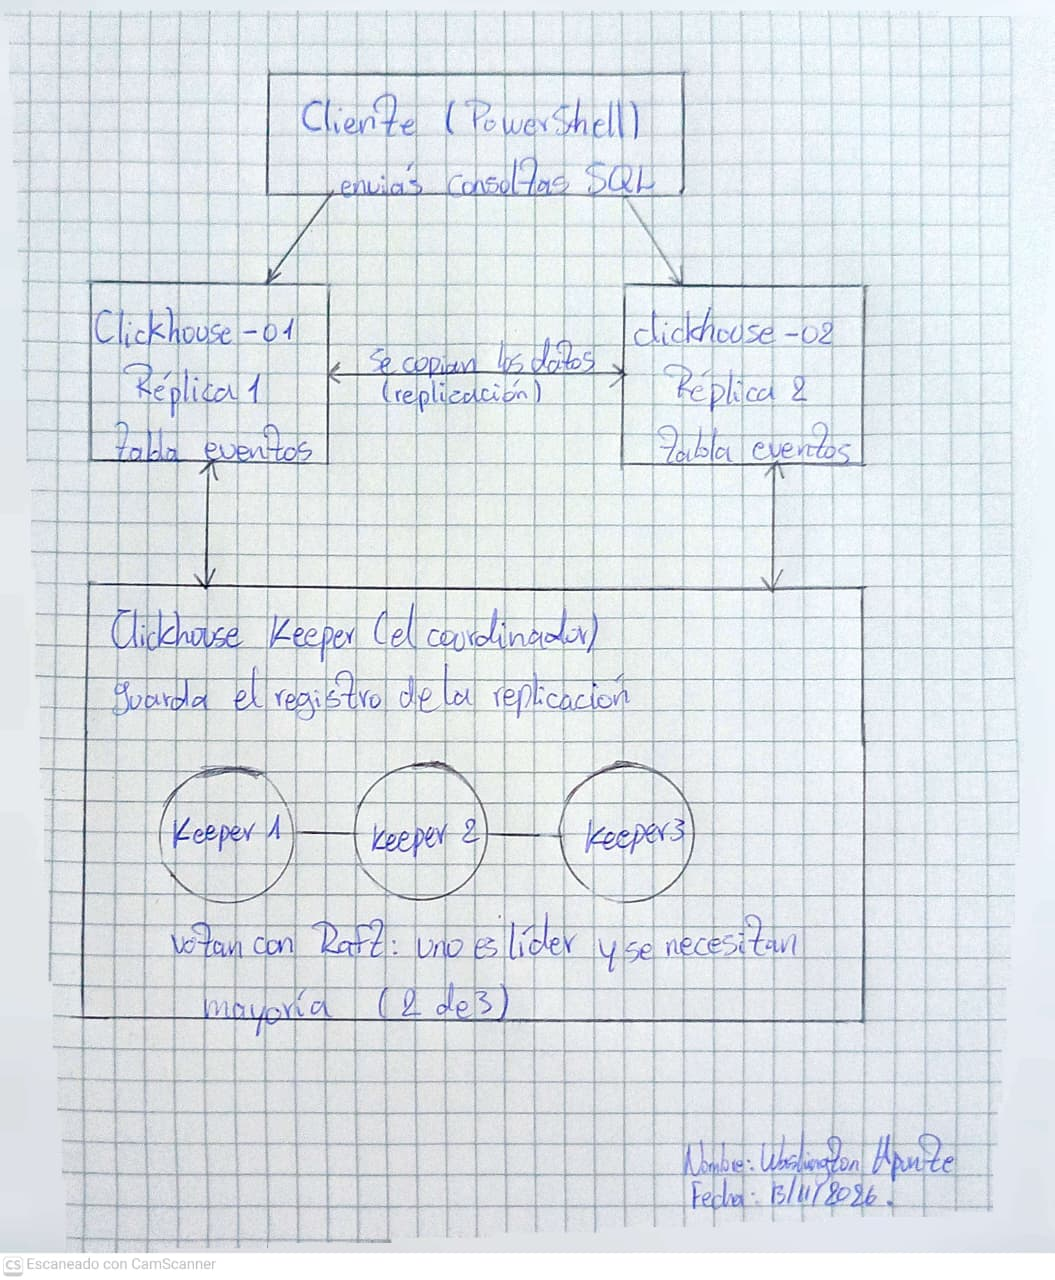
\includegraphics[width=0.7\linewidth]{anexo-a-bosquejo.jpg}
  \caption{Primer bosquejo a mano de la arquitectura (13/11/2026).}
  \label{fig:bosquejo}
\end{figure}

\section{Capturas de lectura de las fuentes}\label{anexo:b}
\begin{figure}[H]
  \centering
  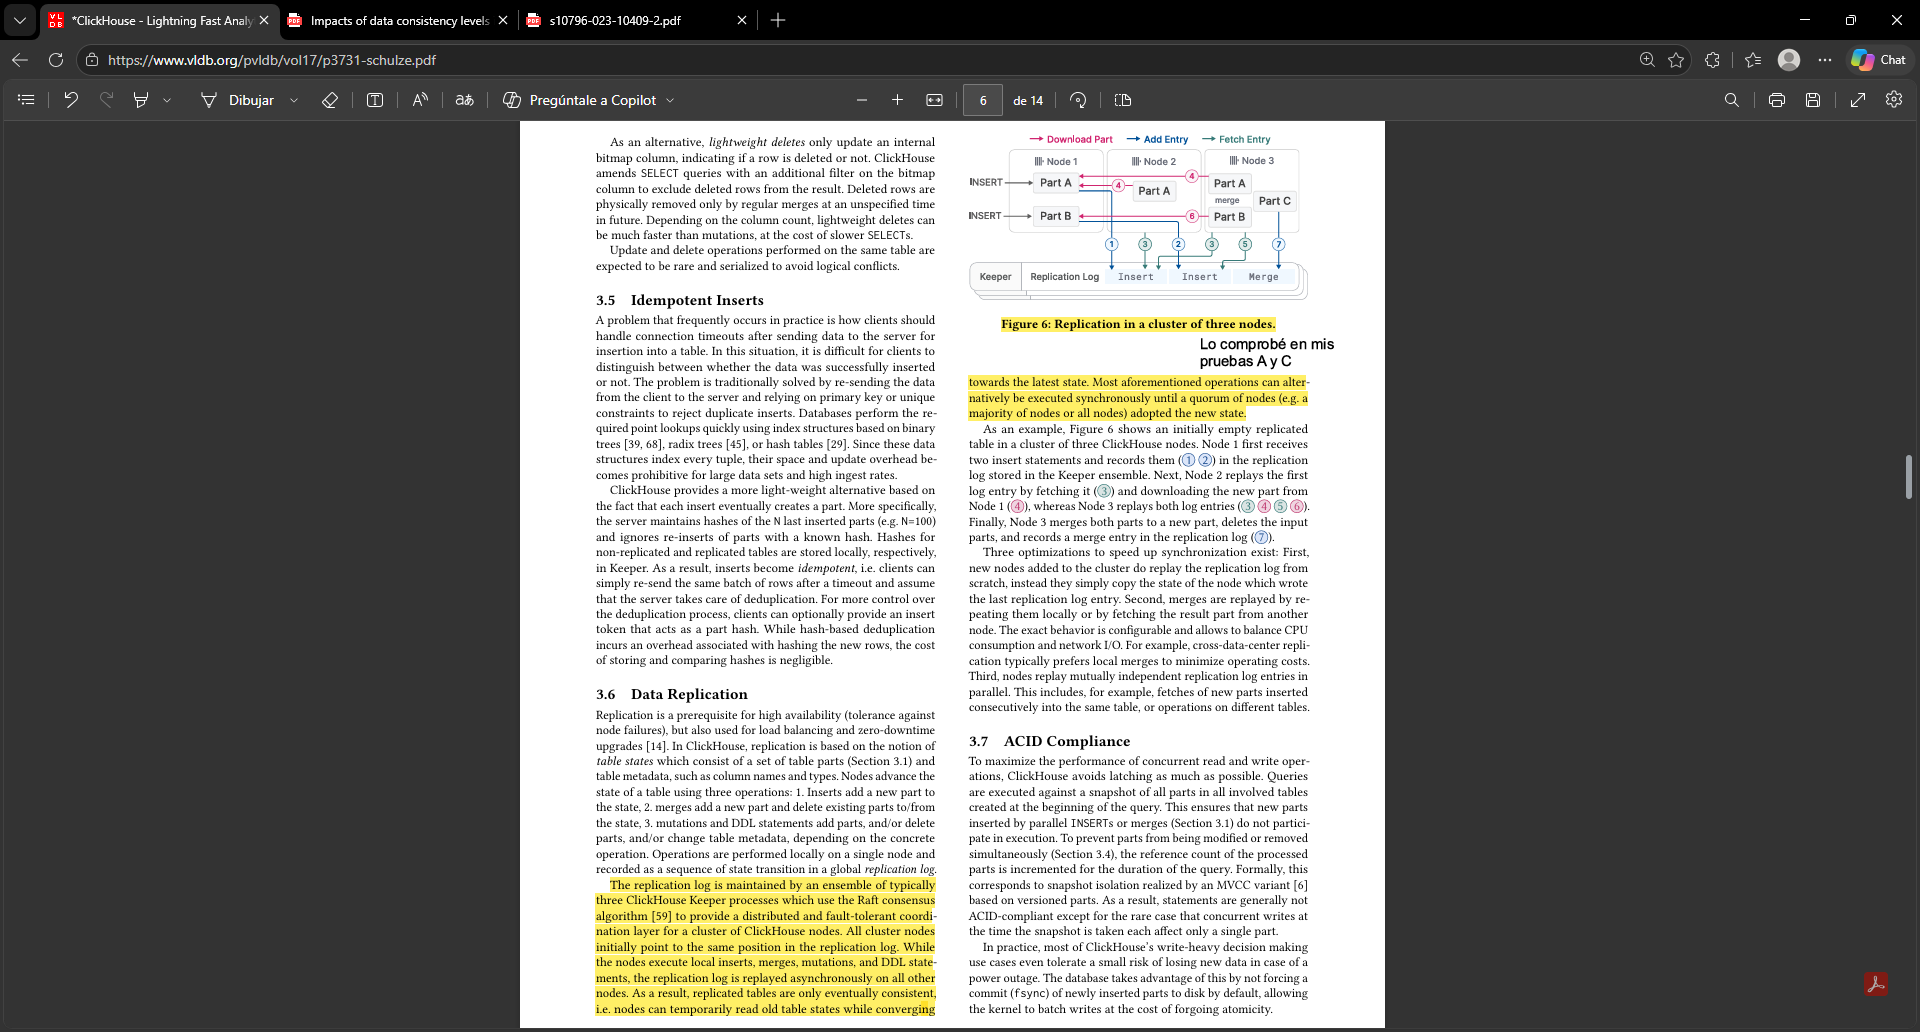
\includegraphics[width=\linewidth]{anexo-b-1-schulze-p3736.png}
  \caption{Lectura de~\cite{schulze2024}, p.~3736: registro de
  replicación en Keeper con Raft y consistencia eventual de las tablas
  replicadas.}
  \label{fig:lectura1}
\end{figure}

\begin{figure}[H]
  \centering
  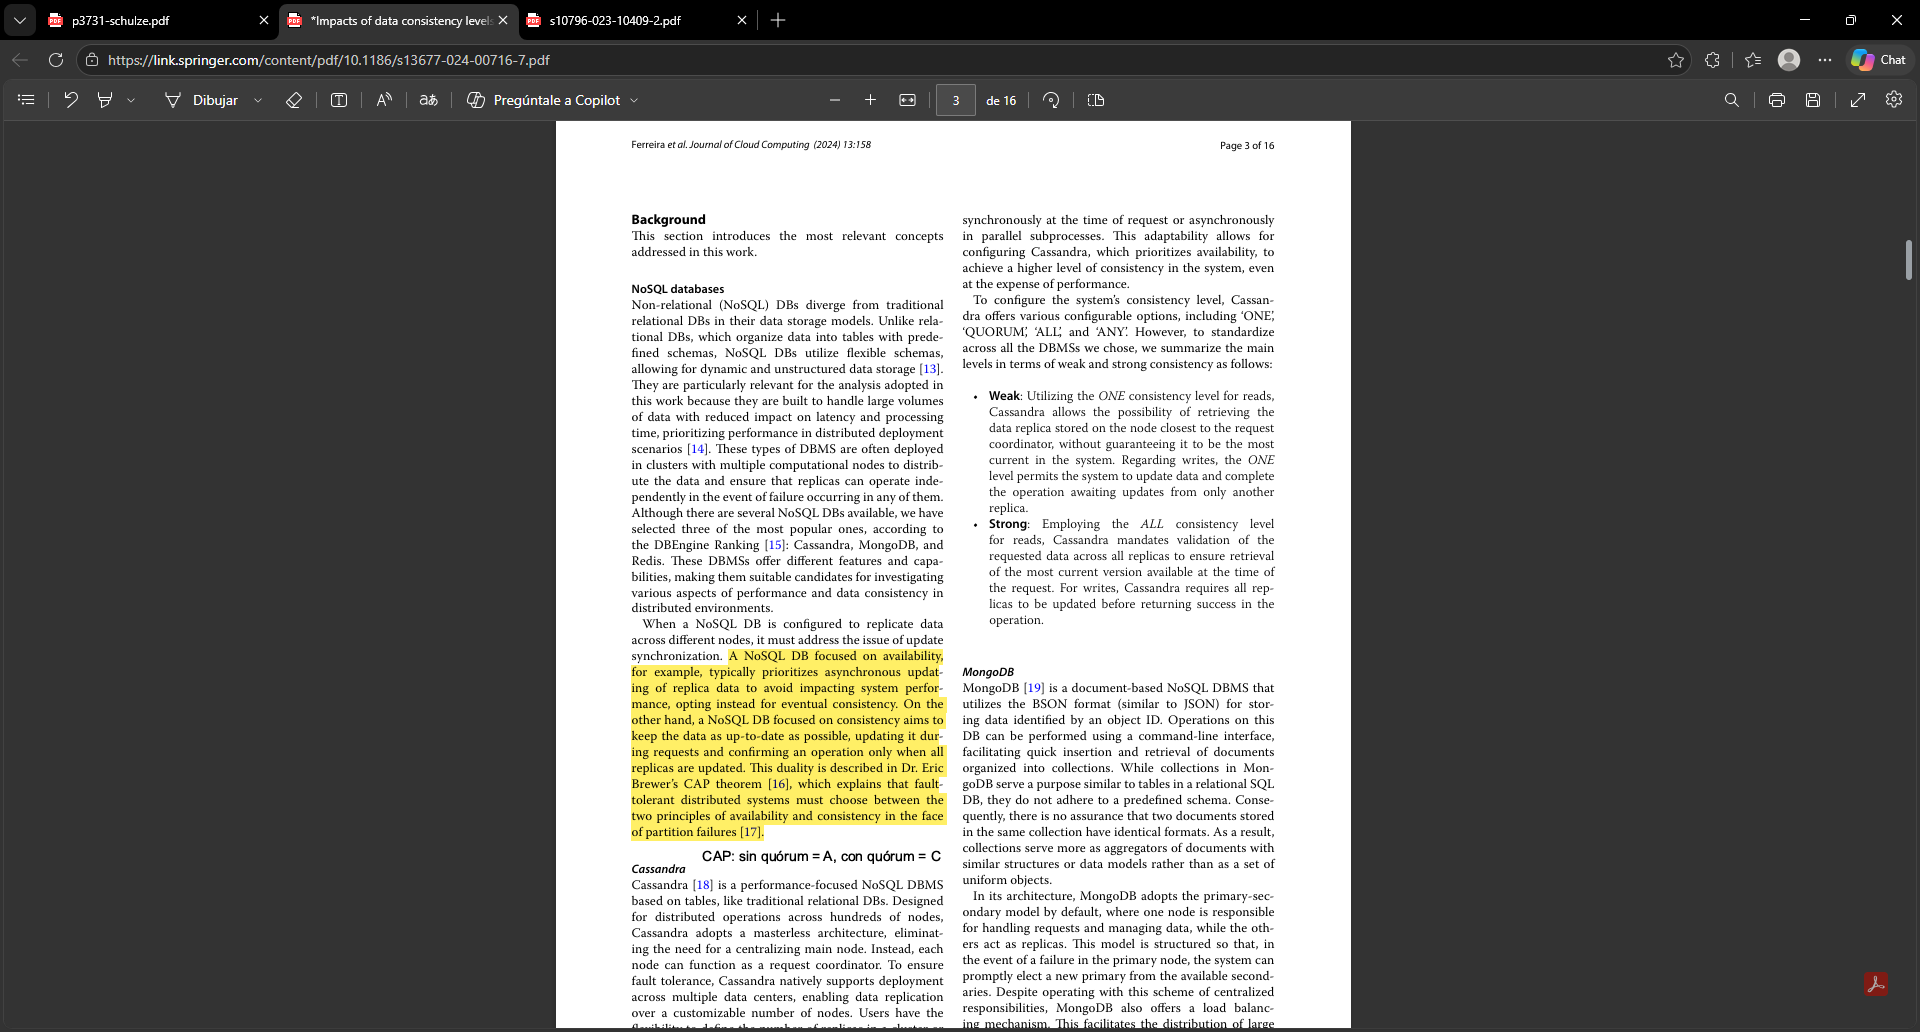
\includegraphics[width=\linewidth]{anexo-b-2-ferreira-p3.png}
  \caption{Lectura de~\cite{ferreira2024}, p.~3: disponibilidad frente a
  consistencia según el teorema CAP.}
  \label{fig:lectura2}
\end{figure}

\begin{figure}[H]
  \centering
  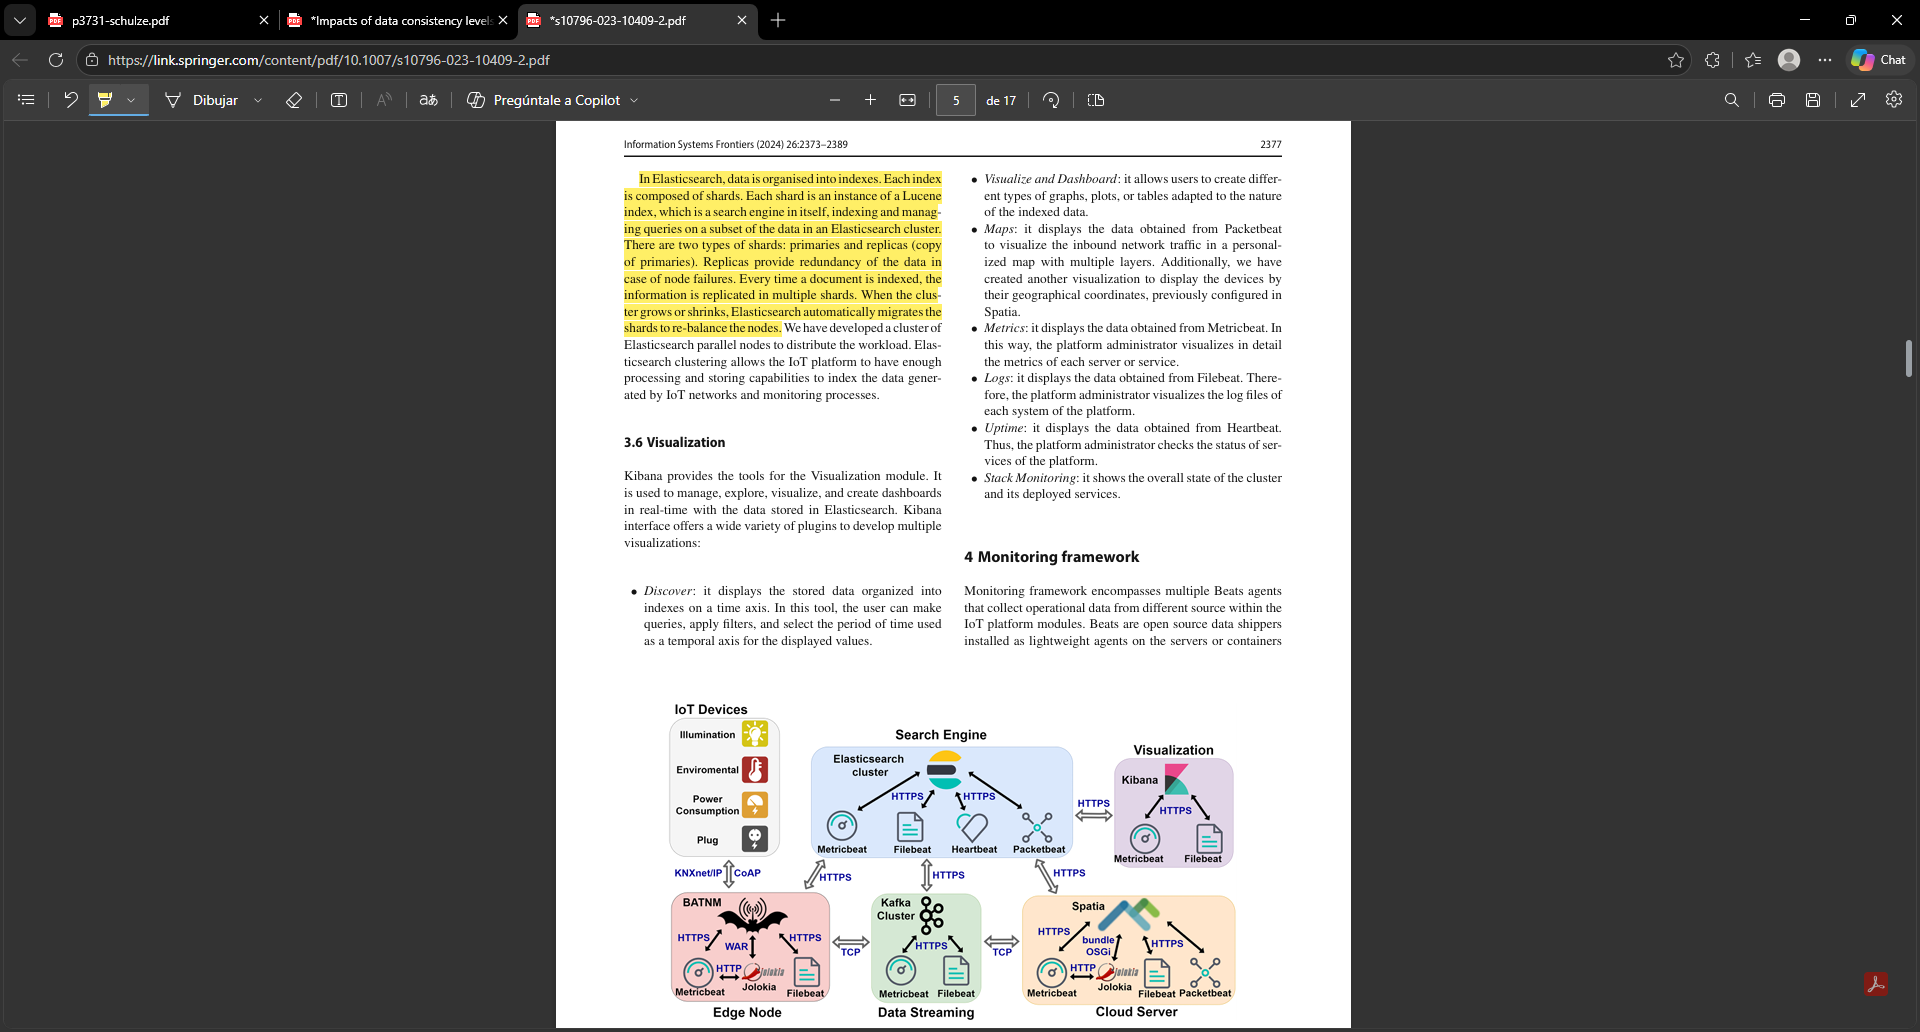
\includegraphics[width=\linewidth]{anexo-b-3-calderon-p2377.png}
  \caption{Lectura de~\cite{calderon2024}, p.~2377: índices, fragmentos
  primarios y réplicas en Elasticsearch.}
  \label{fig:lectura3}
\end{figure}
\end{appendices}

\end{document}
